\subsection{General Results}

We ran the experiment with values of k-gram values of $k=\{3,4,5\}$ and 
total cluster values of $n=\{5,6,7,8,9\}$.
Many of our clusters only have a few data points in them,
so for simplicity we filter all of our results to the clusters that have
100 or more data points.
For the purposes of our results, we only show plots dealing with genres,
as they deal directly with our hypotheses.
Plots dealing with artists and decades, while referenced here,
are in the appendix.

We examined how well the data separates the most frequently occurring values
across genre labels, artists, and decades.
Unfortunately, other than a few exceptions, our clustering method appears to ineffective 
in separate the data along any of those dimensions, no matter the value of $n$ or $k$.

\begin{figure*}[ht]
    \centering
    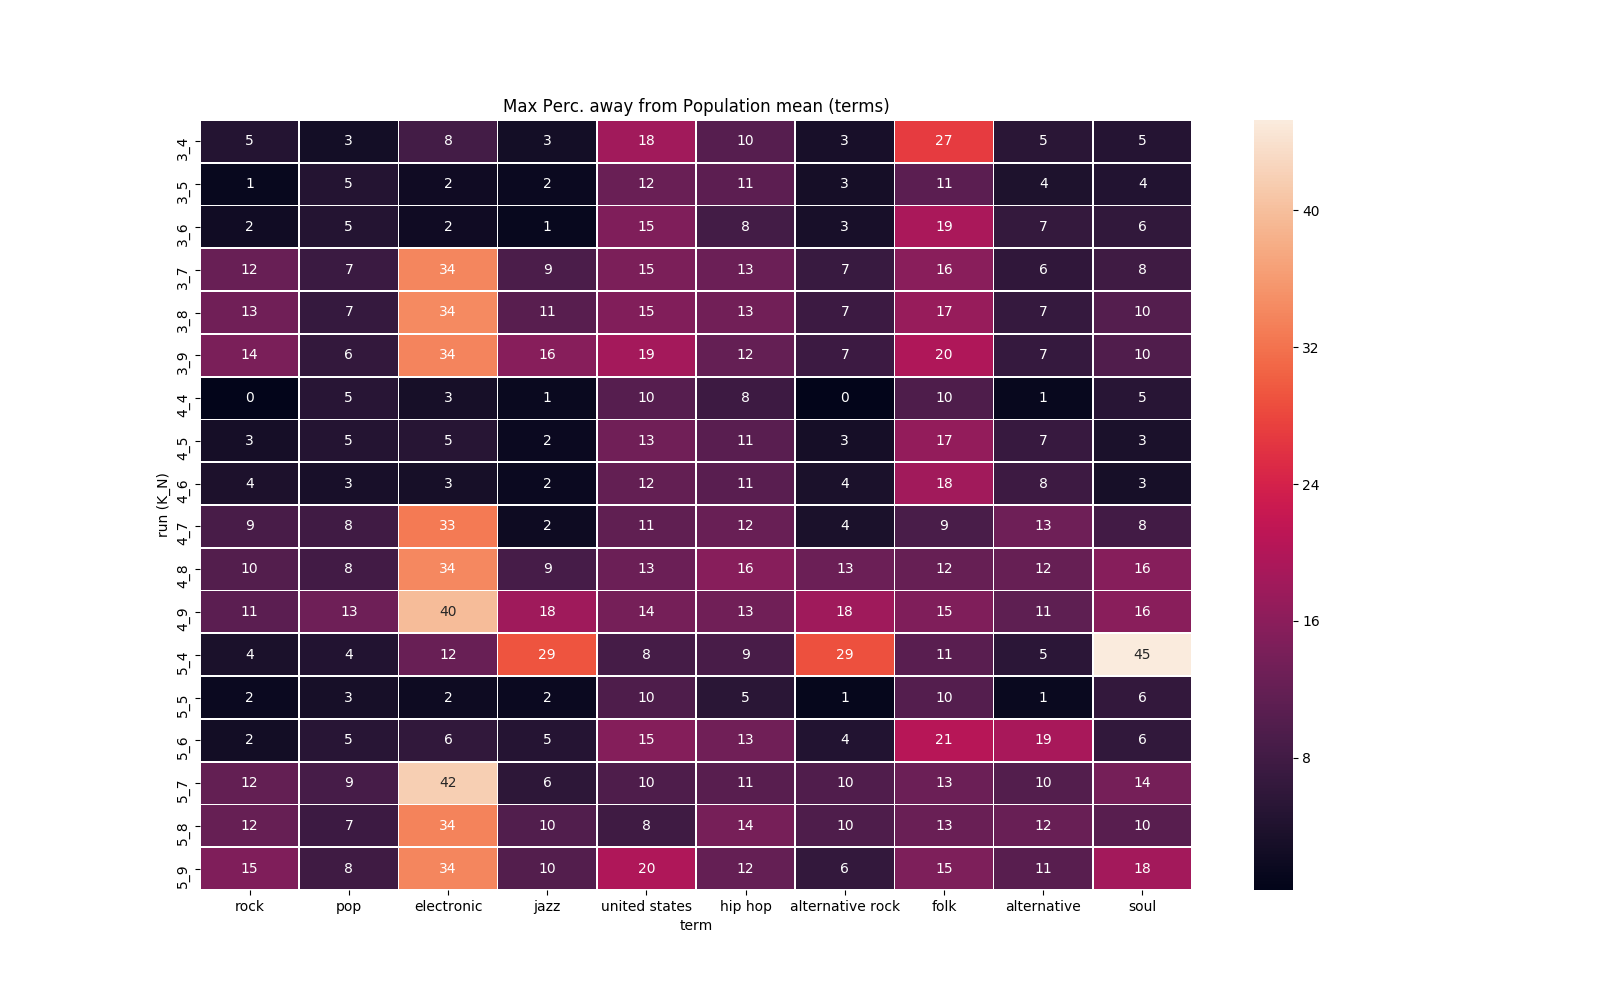
\includegraphics[width=1.2\textwidth]{perc_away_terms}
    \caption{Maximum difference between clusters and population}
    \label{fig:all}
\end{figure*}

We used a few different measures to determine how well clusters separated along genre, year, or artist.
All of the measures are summaries of a run's clusters, and compares against the entire dataset's counts.
We include the standard deviation of variable counts across each run's clusters,
the highest number of standard deviations away from the population count in a run,
and the highest difference in a run between a cluster's portion (in percentage) to the portion in the population.
These measures are all intended to detect if there are clusters that dramatically under or over represent a particular variable,
which would indicate the our clustering separates the variable well.

The results appear fairly noisy, without many discernible patterns.
Electronica music separates well when cluster sizes are $n=\{7,8,9\}$ (See figure~\ref{fig:all})
and 1940s music separates well when cluster sizes are $n=\{4,5,6\}$.

Artists terms in general seem to separate well (See Appendix), with the difference in percentages being
above 100\% of the population in most cases.
However, it should be noted that with artists,
the population frequency is very low (highest is about 0.1\%),
so even a cluster with 100 data points and a single occurrence of the artist will be 900\%
of the population frequency.
There are similar problems with the earlier decades being underrepresented, as can be seen above.

\subsection{K=5, N=4}

Across variables, when $k=5$ and $n=4$, clustering appears to separate better than normal.
So we will look at this cluster in a bit more depth.

\begin{figure*}[ht]
    \centering
    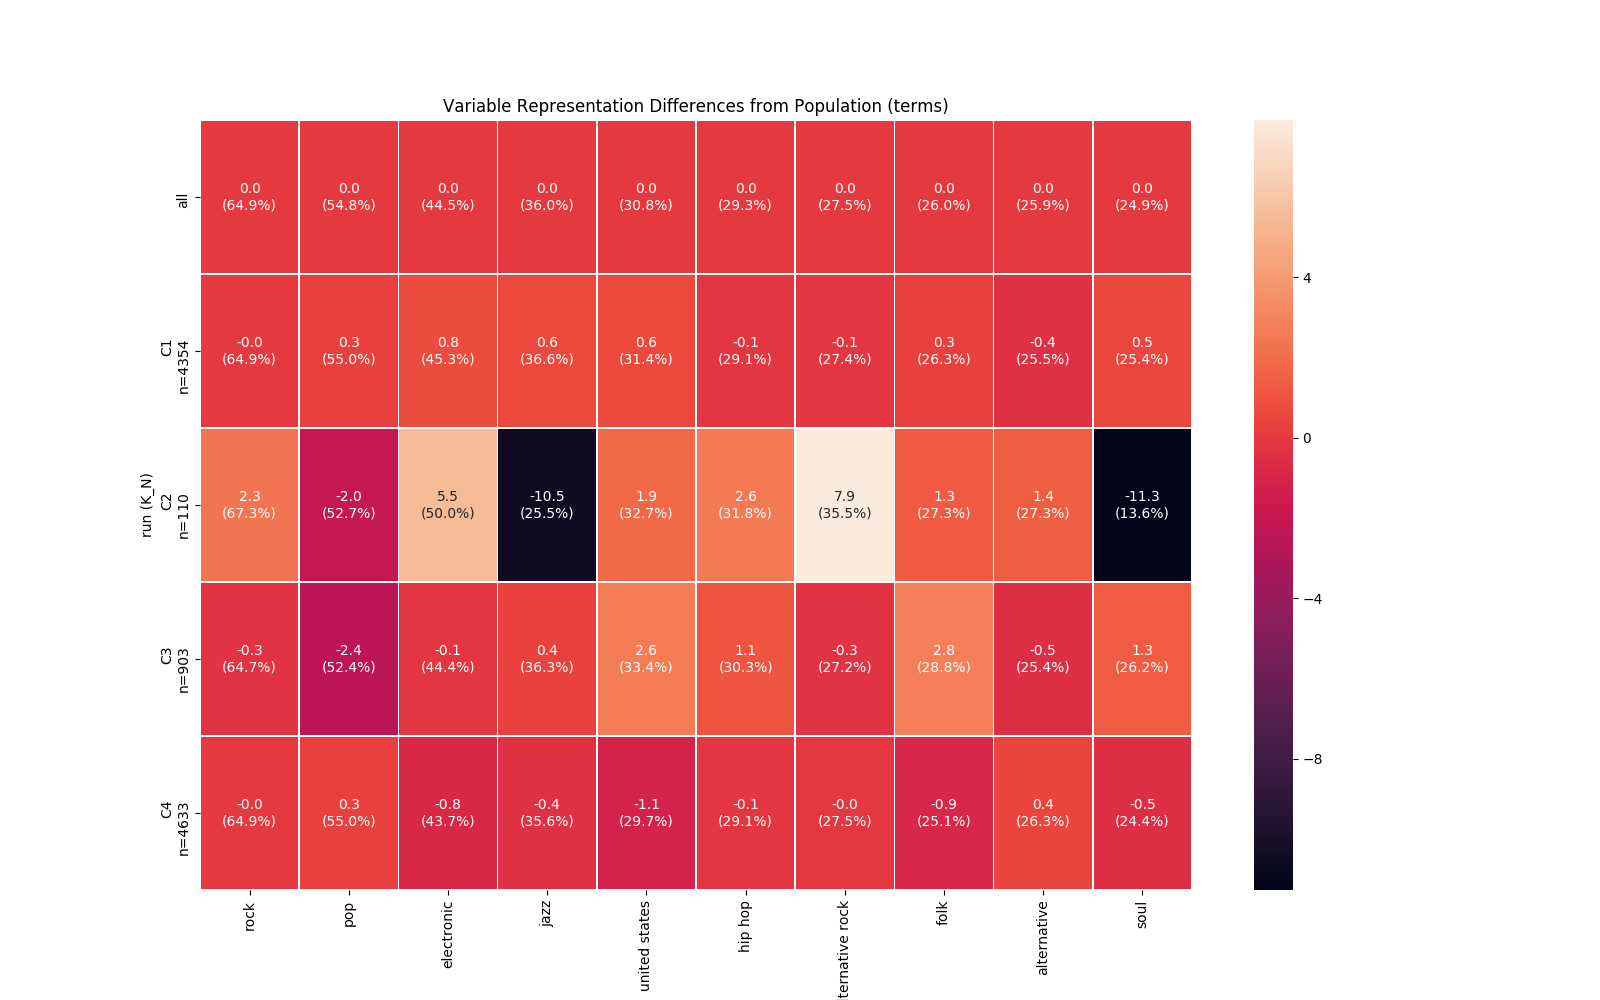
\includegraphics[width=1\textwidth]{terms_cluster}
    \caption{Population vs. Clustering with $k=5$ and $n=4$}
    \label{fig:cluster}
\end{figure*}

Figure~\ref{fig:cluster} show how the clusters are distributed for this run.
There are some stark outliers in how variables are represented between clusters,
such as Jazz, Alternative Rock, and soul in $C2$.
We think that much of this is due to sample size.
$C2$ only has 110 data points, which is much smaller than the other clusters.
The larger clusters are more uniformly distributed across all the variables,
which suggests that the abberations in $C2$ are due mainly to sample size.

